\documentclass[tikz,border=4pt]{standalone}
\usepackage{pgfplots}
\pgfplotsset{compat=1.18}
\begin{document}
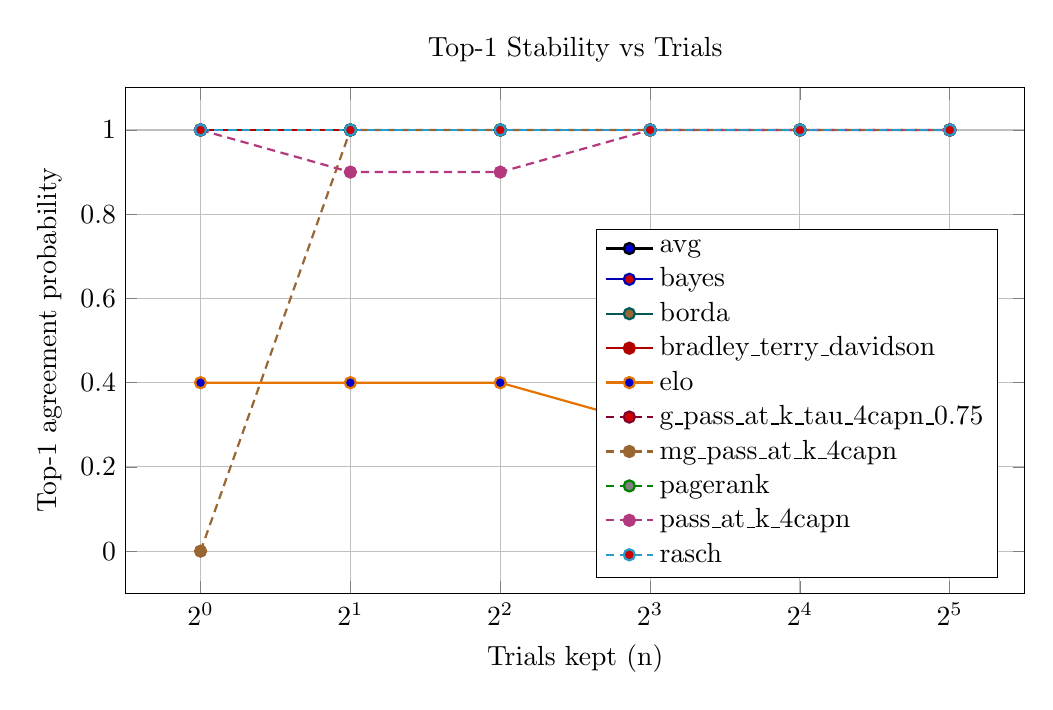
\begin{tikzpicture}
\begin{axis}[
width=13cm,
height=8cm,
title={Top-1 Stability vs Trials},
xlabel={Trials kept (n)},
ylabel={Top-1 agreement probability},
grid=both,
legend pos=south east,
legend cell align=left,
xmode=log, log basis x=2,
]
\addplot+[mark=*, thick, color=black] coordinates {(1,1) (2,1) (4,1) (8,1) (16,1) (32,1)};
\addlegendentry{avg}
\addplot+[mark=*, thick, color=blue!70!black] coordinates {(1,1) (2,1) (4,1) (8,1) (16,1) (32,1)};
\addlegendentry{bayes}
\addplot+[mark=*, thick, color=teal!70!black] coordinates {(1,1) (2,1) (4,1) (8,1) (16,1) (32,1)};
\addlegendentry{borda}
\addplot+[mark=*, thick, color=red!70!black] coordinates {(1,1) (2,1) (4,1) (8,1) (16,1) (32,1)};
\addlegendentry{bradley\_terry\_davidson}
\addplot+[mark=*, thick, color=orange!90!black] coordinates {(1,0.4) (2,0.4) (4,0.4) (8,0.3) (16,0.3) (32,0.2)};
\addlegendentry{elo}
\addplot+[mark=*, thick, color=purple!70!black] coordinates {(1,1) (2,1) (4,1) (8,1) (16,1) (32,1)};
\addlegendentry{g\_pass\_at\_k\_tau\_4capn\_0.75}
\addplot+[mark=*, thick, color=brown!80!black] coordinates {(1,0) (2,1) (4,1) (8,1) (16,1) (32,1)};
\addlegendentry{mg\_pass\_at\_k\_4capn}
\addplot+[mark=*, thick, color=green!50!black] coordinates {(1,1) (2,1) (4,1) (8,1) (16,1) (32,1)};
\addlegendentry{pagerank}
\addplot+[mark=*, thick, color=magenta!70!black] coordinates {(1,1) (2,0.9) (4,0.9) (8,1) (16,1) (32,1)};
\addlegendentry{pass\_at\_k\_4capn}
\addplot+[mark=*, thick, color=cyan!80!black] coordinates {(1,1) (2,1) (4,1) (8,1) (16,1) (32,1)};
\addlegendentry{rasch}
\end{axis}
\end{tikzpicture}
\end{document}
